\documentclass[cs4size,a4paper]{ctexart}   
%==================== 数学符号公式 ============
\usepackage{amsmath}                 % AMS LaTeX宏包
\usepackage[style=1]{mdframed}
\usepackage{amsthm}
\usepackage{amsfonts}
\usepackage{mathrsfs}                % 英文花体字 体
\usepackage{bm}                      % 数学公式中的黑斜体
\usepackage{bbding,manfnt}           % 一些图标,如 \dbend
\usepackage{lettrine}                % 首字下沉,命令\lettrine
\def\attention{\lettrine[lines=2,lraise=0,nindent=0em]{\large\textdbend\hspace{1mm}}{}}
\usepackage{longtable}
\usepackage[toc,page]{appendix}
\usepackage{geometry}                % 页边距调整
\geometry{top=3.0cm,bottom=2.7cm,left=2.5cm,right=2.5cm}
%====================公式按章编号==========================
\numberwithin{equation}{section}
\numberwithin{table}{section}
\numberwithin{figure}{section}
%================= 基本格式预置 ===========================
\usepackage{fancyhdr}
\pagestyle{fancy}
\fancyhf{}  
\fancyhead[C]{\zihao{5}  \kaishu 北邮SDN大赛报告模板}
\fancyfoot[C]{~\zihao{5} \thepage~}
\renewcommand{\headrulewidth}{0.65pt} 
\CTEXsetup[format={\centering\bfseries\zihao{-2}},name={第, 章}]{section}
\CTEXsetup[nameformat={\bfseries\zihao{3}}]{subsection}
\CTEXsetup[nameformat={\bfseries\zihao{4}}]{subsubsection}
%================== 图形支持宏包 =========================
\usepackage{subfigure}
\usepackage{graphicx}                % 嵌入png图像
\usepackage{color,xcolor}            % 支持彩色文本、底色、文本框等
\usepackage{hyperref}                % 交叉引用
\usepackage{caption}
\captionsetup{figurewithin=section}
%==================== 源码和流程图 =====================
\usepackage{listings}                % 粘贴源代码
\usepackage{xcolor}
\usepackage{color}
\definecolor{dkgreen}{rgb}{0,0.6,0}
\definecolor{gray}{rgb}{0.5,0.5,0.5}
\definecolor{mauve}{rgb}{0.58,0,0.82}
 \usepackage{xcolor}
 \lstset{
  %行号
    numbers=left,
    %背景框
    framexleftmargin=8mm,
    frame=none,
     %背景色
    %backgroundcolor=\color[rgb]{1,1,0.76},
     backgroundcolor=\color[RGB]{245,245,244},
     %样式
   keywordstyle=\bf\color{blue},
   identifierstyle=\bf,
    numberstyle=\color[RGB]{0,192,192},
    commentstyle=\it\color[RGB]{0,96,96},
   stringstyle=\rmfamily\slshape\color[RGB]{128,0,0},
   %显示空格
    showstringspaces=false
 }


%--------------------
\hypersetup{hidelinks}
\usepackage{booktabs}  
\usepackage{shorttoc}
\usepackage{tabu,tikz}
\usepackage{float}

\usepackage{multirow}



\tabcolsep=1ex
\tabulinesep=\tabcolsep
\newlength\tikzboxwidth
\newlength\tikzboxheight
\newcommand\tikzbox[1]{%
        \settowidth\tikzboxwidth{#1}%
        \settoheight\tikzboxheight{#1}%
        \begin{tikzpicture}
        \path[use as bounding box]
                (-0.5\tikzboxwidth,-0.5\tikzboxheight)rectangle
                (0.5\tikzboxwidth,0.5\tikzboxheight);
        \node[inner sep=\tabcolsep+0.5\arrayrulewidth,line width=0.5mm,draw=black]
                at(0,0){#1};
        \end{tikzpicture}%
        }

\makeatletter
\def\hlinew#1{%
  \noalign{\ifnum0=`}\fi\hrule \@height #1 \futurelet
   \reserved@a\@xhline}
   
\newcommand{\tabincell}[2]{\begin{tabular}{@{}#1@{}}#2\end{tabular}}%

\usepackage{subfigure}

\usepackage{CJK}
\usepackage{ifthen}


\usepackage{graphicx} 
\newcommand{\HRule}{\rule{\linewidth}{0.5mm}}

\newtheorem{Theorem}{定理}
\newtheorem{Lemma}{引理} 
%%使得公式随章节自动编号
\makeatletter
\@addtoreset{equation}{section}
\makeatother
\renewcommand{\theequation}{\arabic{section}.\arabic{equation}}

%-------------------------
	
\usepackage{pythonhighlight}
\usepackage{tikz}                    
\usepackage{tikz-3dplot}
\usetikzlibrary{shapes,arrows,positioning}
%===================   正文开始    ===================
\begin{document}
\bibliographystyle{gbt7714-2005}     %论文引用格式
%===================  定理类环境定义 ===================
\newtheorem{example}{例}              % 整体编号
\newtheorem{algorithm}{算法}
\newtheorem{theorem}{定理}            % 按 section 编号
\newtheorem{definition}{定义}
\newtheorem{axiom}{公理}
\newtheorem{property}{性质}
\newtheorem{proposition}{命题}
\newtheorem{lemma}{引理}
\newtheorem{corollary}{推论}
\newtheorem{remark}{注解}
\newtheorem{condition}{条件}
\newtheorem{conclusion}{结论}
\newtheorem{assumption}{假设}
%==================重定义 ===================
\renewcommand{\contentsname}{目录}     
\renewcommand{\abstractname}{摘要} 
\renewcommand{\refname}{参考文献}     
\renewcommand{\indexname}{索引}
\renewcommand{\figurename}{图}
\renewcommand{\tablename}{表}
\renewcommand{\appendixname}{附录}
\renewcommand{\proofname}{证明}
\renewcommand{\algorithm}{算法} 
%============== 封皮和前言 =================
\begin{titlepage}

\begin{center}


% Upper part of the page

\includegraphics[width=0.65\textwidth]{figure/logo}\\[1cm]    

\textsc{\LARGE Beijing Univers of Posts and telcom}\\[1.5cm]

\textsc{\Large Preliminary report}\\[0.5cm]


% Title
\HRule \\[0.4cm]
{ \huge \bfseries SDN初赛报告模板}\\[0.4cm]

\HRule \\[1.5cm]

% Author and supervisor
\begin{minipage}{0.4\textwidth}
\begin{flushleft} \large
\emph{Author:}\\
Li \textsc{Yingmin}
\end{flushleft}
\end{minipage}
\begin{minipage}{0.4\textwidth}
\begin{flushright} \large
\emph{Supervisor:} \\
Dr.~Mark \textsc{Brown}
\end{flushright}
\end{minipage}

\vfill

% Bottom of the page
{\large \today}

\end{center}

\end{titlepage}


%%=============设计(论文)任务书===========
%\begin{center}
%\zihao{-2}\textbf{\songti 本科生毕业设计(论文)任务书} 
%\end{center}
%\smallskip
%\renewcommand{\arraystretch}{1.3}
%\begin{tabular}{lll}
%\zihao{4} \textbf{\songti 学生姓名: 曹宇} & & \zihao{4} \textbf{\songti 专业班级:\quad\quad 船海1006班} \\ 
%\zihao{4} \textbf{\songti 指导教师:徐海祥}&\makebox [3cm] & \zihao{4} \textbf{\songti 工作单位:\quad 武汉理工大学} \\ 
%\end{tabular}\\
%\begin{tabular}{lll}
%\zihao{4} \textbf{\songti 设计(论文)题目:}& \zihao{4} \textbf{\songti  武汉理工本科论文\LaTeX 模板 } &\\ 
%\zihao{4} \textbf{\songti 设计(论文)主要内容:} \\
%\end{tabular} \\ 
%\begin{enumerate}
%\item \LaTeX 环境的配置
%\item 主要字体的控制和数学公式的选用
%\item 图表和代码的粘贴
%\end{enumerate}
%\begin{tabular}{ll}
%\zihao{4} \textbf{\songti 要求完成的主要任务:}
%\end{tabular} \\ 
%\begin{enumerate}
%\item 选择合适的\TeX 编辑系统
%\item 学习如何使用控制代码完成排版
%\item 合理的安排学习和科研的时间来发展自己兴趣爱好
%\end{enumerate}
%\begin{tabular}{ll}
%\zihao{4} \textbf{\songti 必读参考资料:}
%\end{tabular}
%\begin{enumerate}
%\item \LaTeX  \quad User Manual
%\item  字体设计的艺术
%\end{enumerate}
%\begin{tabular}{lll}
%\zihao{4} \textbf{\songti 指导教师签名: }&\makebox [4cm]& \zihao{4} \textbf{\songti 系主任签名:} \\
%& & \zihao{4} \textbf{\songti 院长签名(章)}
%\end{tabular}
%\thispagestyle{empty}
%\clearpage
%%==========本科生毕业设计(论文)开题报告  =============
%\begin{center}
%\zihao{-2} \textbf{\songti 武汉理工大学}\\
%\zihao{-2} \textbf{\songti 本科生毕业设计(论文)开题报告} 
%\end{center}
%\begin{tabular}{|l|}
%\hline \rule[-2ex]{0pt}{5.5ex} \makebox[13.5cm][l]{\zihao{4} \heiti 1、目的及意义(含国内外的研究现状分析) } \\ 
%\quad \LaTeX 是国际通行的科技论文排版软件,国际上科研机构和大学都采用它写作\\
%\quad 国内著名高校都有自己的本科生\LaTeX 模板供毕业生使用\\
%\quad 但是武汉理工大学还没有本科生\LaTeX 模板可以参考\\
%\quad 人类的价值在于创造而不是索取 \\
%\hline \rule[-2ex]{0pt}{5.5ex}  \zihao{4} \heiti
%2、基本内容和技术方案\\ 
%\quad 采用GITHUB托管降低代码维护成本\\
%\quad 加入在线\TeX 编辑器的使用简介 \\
%\quad 授人以渔,注重方法和理念的引导\\
%\hline \rule[-2ex]{0pt}{5.5ex}  \zihao{4} \heiti
%3、进度安排 \\ 
%\quad 离 deadline 两个月吃喝玩乐 \\
%\quad 离 deadline 一个月吃喝玩乐 \\
%\quad 离 deadline 半个月吃喝玩乐 \\
%\quad 离 deadline 一个星期狂写论文 \\
%\hline \rule[-2ex]{0pt}{5.5ex} \zihao{4} \heiti
%4、指导教师意见 \\ 
%\quad 曹宇同学是个好同志\\
%\quad 曹宇同志是个好同学\\
%\quad 本表格是支持跨页的长表格,你可以复制上面的内容进行测试\\
%\quad 具体方法是将tabular改为 longtable然后再编译\\
%\makebox[10cm][r]指导教师签名:\\
%\makebox[12cm][r]\quad 年\quad 月\quad 日\\
%\hline 
%\end{tabular} 
%\thispagestyle{empty}

\pagestyle{plain}
\pagenumbering{Roman}
% !TEX root = ../thesis_phd.tex  %宏命令,编译的时候自动链接到主文件
%
\pdfbookmark[0]{Abstract}{Abstract}
\chapter*{Abstract}
\label{sec:abstract}
\vspace*{-10mm}

\blindtext



\pagestyle{empty}
\tableofcontents 
\thispagestyle{empty}
%============== 论文正文   =================
\pagestyle{fancy}
\pagenumbering{arabic}
\section{\LaTeX 入门简介}
\LaTeX 是国际通行的格式化排版系统,在数学界和计算机科学界有着极为广泛的运用。学习\LaTeX 排版规则是每一个科研人员熟悉科研论文格式化写作,提高论文质量的不二之选。
\subsection{编辑环境}
编译环境由编辑器和编译器两个部分组成, 编辑器的功能和我们常见的写字板差不多,它能够了方便我们处理\TeX 源码明确彼此之间的篇章关系,从而提高排版效率。而编译器则是将\TeX 语言转化为计算机能够理解的二进制代码并最终呈现为我们能够阅读的PDF文档,他们之间相互分工共同完成排版任务。
\subsubsection{编辑器}
编辑器的种类非常多,有“所见即所得”的\textbf{LyX},也有Linux向的\textbf{Emacs}和\textbf{Vim},还有伪geek向的\href{http://www.sublimetext.com/}{\textbf{Sublime Text}},而我自己则偏爱IDE向的
\href{http://texstudio.sourceforge.net/}{\textbf{\TeX Studio}}.它有着一些令我爱不释手的特性,如:
\begin{enumerate}
\item 清晰的组织结构,你可以在屏幕左侧看到他们
\item 便捷的自动补充功能,只要输入命令的一部分就能够完成撰写
\item 合理的宏包查看方式,右键菜单中可以找到宏包的文档
\item 贴心的实用工具,矩阵插入助手,表格编辑助手等
\end{enumerate}

每个人都可以选择自己顺手的编辑器,如果你真的非常懒不愿意在如此多的选择中做出一个抉择那么编译器中自带的\textbf{\TeX Works}也是一个不错的选择。
\subsubsection{编译器}
编译器一般存在于封装了宏包的各种\TeX 发行包中,按照宏包数量的多少从几十兆字节到若干个G都有。按照操作系统平台的不同,比较流行的发行包有\TeX Live,pro\TeX t和Mac\TeX . 在Windows 平台或者 Linux 平台上常用的是\href{https://www.tug.org/texlive/}{\TeX Live},如果您需要从网络上下载请选择\href{https://www.tug.org/texlive/acquire-iso.html}{ISO镜像}进行下载。国内知名大学均有镜像FTP下载站,通过他们你可以获得这个3GB左右的ISO包,安装它可以免去您下载各类宏包和寻找文档的麻烦。
\subsection{尝试编译}
\subsubsection{Windows}
安装并设置完毕软件环境之后,就可以尝试对于本论文进行编译工作。打开文件夹中的\verb|thesis.tex| 文件,将默认编译器设置为Xe\LaTeX(\TeX Studio 中依次点击Options - Configure TeXstudio - Built - Default Complier 内选择Xe\LaTeX ,\TeX works 则可以选择左上角的下拉菜单在其中找到Xe\LaTeX ),点击编译按钮就可以开始编译过程了。

正常编译结束之后,文件夹中会出现一个\verb|thesis.pdf|的文件同时编辑器也会自动打开该文件生成一个精美的预览。你可以对比自己编译出来的成果与本文件之间的差异,来确定编译器和编辑器是否已经设置妥当。
\subsubsection{Mac OS X}

在OS X系统下,由于系统内字体的区别,本模板会遇到一些编译上的问题。 我们需要手动调整一下字体的设置,以正常编译模板, 具体修改方式可以参见\href{http://www.zhihu.com/question/22906637}{知乎问答}。 

问答的第四步可能需要一些修改,
\begin{verbatim}
	cd /usr/local/texlive/2014/texmf-dist/tex/texlive/ctex
\end{verbatim}

\subsubsection{Linux}
本模板在Ubuntu 14.04 以及12.04 长期稳定支持版上均编译通过。

\subsection{简单步骤}
先\href{https://www.tug.org/texlive/acquire-iso.html}{下载}\TeX 发行包(内含编译器和相关宏包及文档),安装这个发行包大概需要20分钟左右的时间,安装期间请关闭杀毒软件以保证组件的顺利注册。
使用自带的编辑器或者下载\href{http://texstudio.sourceforge.net/}{\textbf{\TeX Studio}},作为默认编辑器使用。打开\verb|thesis.tex|,并设置编译器为Xe\LaTeX 再进行一次编译。如果遇到无法编译的问题请注意以下技术细节:

相关路径设置是否正确,在\textbf{\TeX Studio}的Options - Configure TeXstudio - Commands 中检查路径,正确的路径\cite{谢琪-203}形式应该类似于

\begin{verbatim}
"D:/Program Files/texlive/2013/bin/win32/latex.exe"
 -src -interaction=nonstopmode %.tex
\end{verbatim}

























      %
\section{开始撰写论文}
在\LaTeX 中论文的组织形式是严格按照结构化写作的方式展开的,章节之间层次分明,段落之间关系紧密。要做到这一点就需要熟悉结构化写作的一般过程,首先需要通过\TeX 命令定义各章节的标题。
\begin{verbatim}
\section{开始撰写论文}              %对应为  第2章 开始撰写论文
\subsection{标题与正文格式控制}     %对应为   2.1 标题与正文格式的控制 
\subsubsection{字体的控制命令}      %对应为   2.1.1 字体的控制命令
\end{verbatim}
由于采用了\verb|ctex|的\verb|article|类作为论文的基本类,所以定义标题的层级最多为二级标题。当你的论文出现三级标题如\verb|2.1.1.1|的时候,请考虑修改文章层级结构以适应格式化排版的要求。(四级标题多出现于书籍以及科技专著中,毕业论文作为文档类其出现此类三级标题的情况较为罕见)。在一个低级标题之后出现的一个高级标题会使得文档当前内容跳出作用域,通过这样的方式整个文章的整体脉络就可以很清晰地显现出来。
\subsection{字体字号的控制}
字体字号的处理是借助了\href{http://mirror.hust.edu.cn/CTAN/language/chinese/ctex/doc/ctex.pdf}{ctex}宏包实现的,仔细阅读该文档你能在中文格式处理方面节省许多时间。在宏包中对于处理字体和字号的方法进行详细的阐述。在我们熟知的排版系统中,形式和内容是一个密不可分的整体,两者相生相伴无法分离。从我们写下一段话,并选中这段话然后再设定字体和字号开始形式已经开始附加到我们想要表达的内容中了。但是在\LaTeX 中,所有的内容(也就是正文及相关附录)是不包含任何关于格式的信息的。这样就做到了形式与内容的彻底分离,是\LaTeX 区别于任何一个排版系统的根本原因。

实现内容与形式的剥离是一个痛苦的过程,我们需要摒弃我们懒惰的直觉并开始高度抽象化的思考,通过这样一个过程等到内容与形式再度统一。
\subsubsection{字体}
根据中文汉字支持宏包ctexart的参考文档,模板中预置的常用字体一共有五种,他们分别是:宋体,黑体,仿宋,楷书, 隶书。对应的控制方式如下:
\begin{center}
\begin{tabular}{ccccc}
\hline \rule[-2ex]{0pt}{5.5ex} { 宋体} & { 黑体} & { 仿宋} & { 隶书} & {楷书} \\ 
\hline \rule[-2ex]{0pt}{5.5ex} \textbackslash songti &\textbackslash  heiti  & \textbackslash fangsong & \textbackslash lishu & \textbackslash kaishu \\ 
\hline 
\end{tabular}  
\end{center}
这些字体基本满足了武汉理工大学本科生毕业论文中所要求的字体的需求。


\subsubsection{字号}
使用\verb|\zihao{4}|命令来规定四号字体,在前面加负号表示小四\verb|\zihao{-4}|.
\subsection{图片及表格的处理}

\subsubsection{在文档中加入图片}
理论上\LaTeX 可以处理各种各样的图片类型从jpeg到bmp,从pdf到eps都是可以接受的图片处理类型。选择合理的图片类型会提高论文的整体观感,使得最终的排版效果更为优良。而其中以无损压缩格式为优先推荐,原生pdf图片,原生eps图片都是最优的选择。如果实在无法找到矢量图,可以退而求其次地采用png图片或者jpeg格式的图片。
\begin{itemize}
\item \textbf{取人玫瑰手留余香}~~~~使用他人图片时记得标注出处和明显的引用。
\item \textbf{掌握一种数据绘图软件}~~~~Python, MATLAB, Mathematica 都是不错的选择
\item \textbf{探索示意图绘制的方法}~~~~指的是流程图,二维或三维线图,推荐Ipe editor, TiKZ, 以及 Microsoft Visio Ink-scape
\end{itemize}
图片插入范例
\begin{figure}[thbp!]
\centering
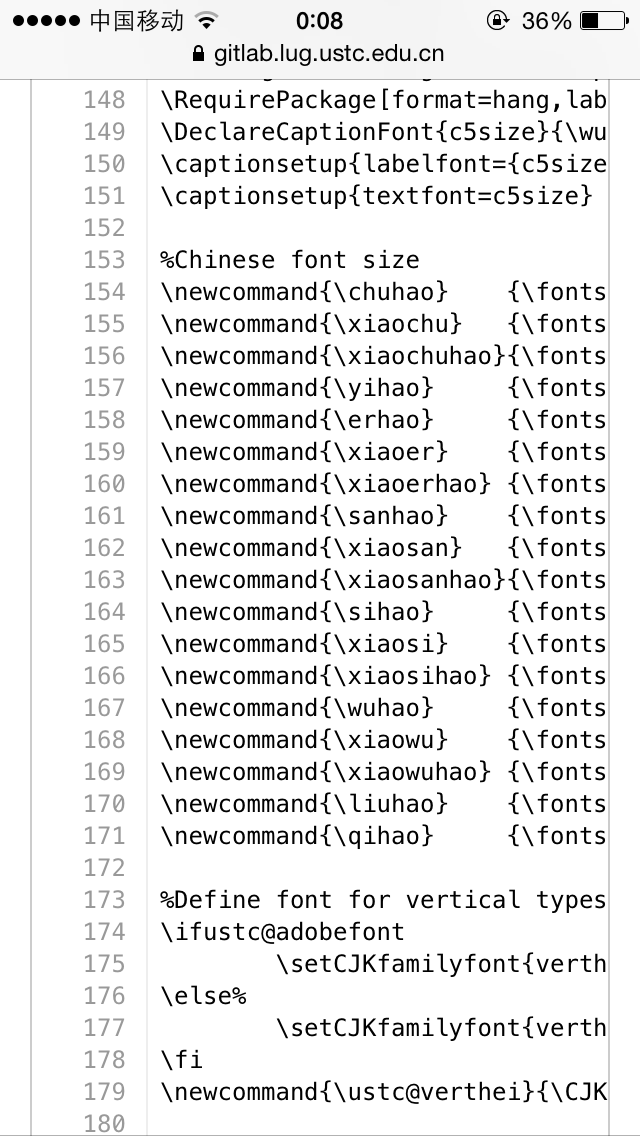
\includegraphics[width=0.4\linewidth]{figure/IMG_1832}
\caption{\LaTeX 字号错误使用范例}
\label{fig:IMG_1832}
\end{figure}

为了插入这样的图片,我们使用了如下的代码:
\begin{verbatim}
\begin{figure}[thbp!]
\centering
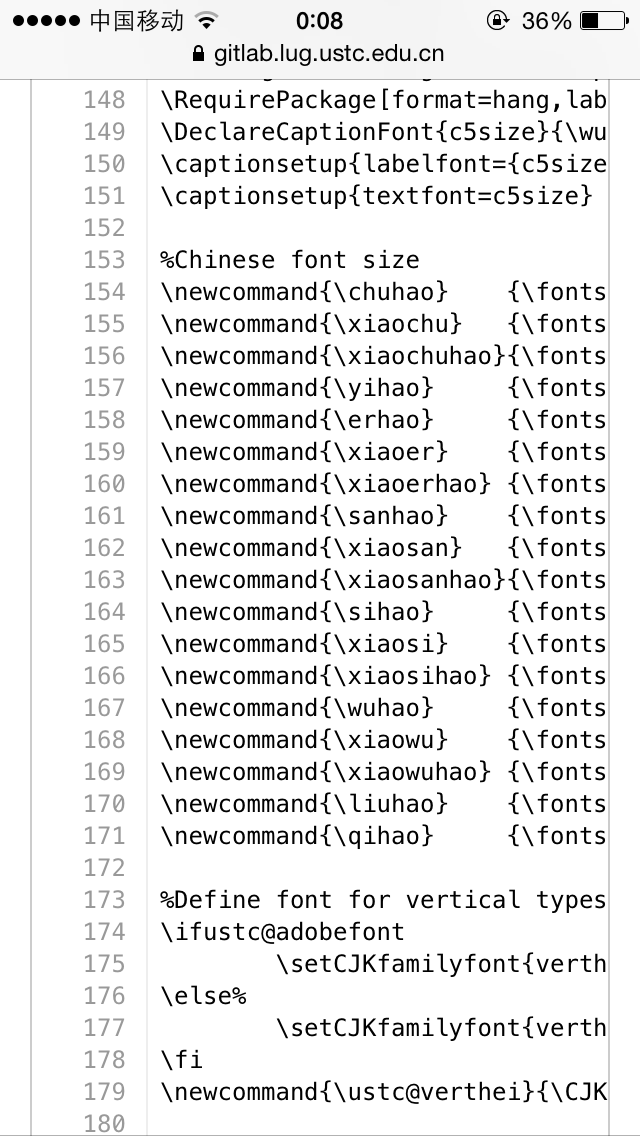
\includegraphics[width=0.6\linewidth]{figure/IMG_1832}
\caption{\LaTeX 字号错误使用范例}
\label{fig:IMG_1832}
\end{figure}
\end{verbatim}
其中第一行的\verb|[thbp!]|是用来规定图片位置的命令\verb|t|表示顶部,\verb|h|表示这里,\verb|b|表示底部,\verb|p|则表示“随便哪儿!”\verb|!|则表示“就是这里!” 在第三行中,规定了图片的尺寸,其方式为限定尺寸宽度为0.6倍行线宽。最后是图片的标题和它的标号,有了它们可以很方便地引用一个图片。

在文档中,虽然我们规定了图片所安放的位置和相对应的顺序,但是图片最终在文档中所呈现的位置和代码中的还是会有差距。这是由于所有的图片实际上都是“浮动” 环境,在设置了图片的大小之后实际上最终的位置还是由文字结束之后可以容纳图片的空间位置所决定的。 如果文档末尾空间不足以填充图片,那么排版系统会自动先将文字填充于这个部分然后再放置我们想要的图片。图片的位置时常让我们感到困惑,如果遇到图片位置的问题可以有几个思路参考:
\begin{itemize}
	\item 更改图片大小,或者宽度。由于大多数情况下我们需要图片等比例缩放,实际上修改宽度和修改图片大小是一样的原理。
	\item 新增一个新的页面,容纳过多的图片。
	\item 合理安排图片的数量,避免做“插图大师”。科研文章都是为了内容服务的,切莫为了字数要求,页数要求而恶意灌图。
\end{itemize}

如图(\ref{fig:IMG_1832})中显示了一个错误的字号显示的方法。
\begin{figure}[h]
\centering
\tdplotsetmaincoords{70}{110}
\begin{tikzpicture}[auto,scale=1,tdplot_main_coords]
\draw[thick,->] (0,0,0) -- (3,0,0) node[anchor=north east]{$x$};
\draw[thick,->] (0,0,0) -- (0,3,0) node[anchor=north west]{$y$};
\draw[thick,->] (0,0,0) -- (0,0,3) node[anchor=south]{$z$};
\draw[thick,->,color=red] (1,0,0)--(1,1.5,0.8) node[midway,name=a]{$ \vec{a} $};
\draw[thick,->,color=red] (1,0,0)--(1,-0.8,1.5) node[midway,name=b]{$ \vec{b} $};
\end{tikzpicture}
\caption{三维向量旋转示意}
\label{fig:3Drot}
\end{figure}

而图(\ref{fig:3Drot})则是用TikZ语言做的图片,比较清晰明了。
\subsubsection{在文档中加入表格}
三线表的使用,见如下代码
\begin{verbatim}
\begin{table}[thbp]
\caption{状态估计算法比较}
\begin{center}
\begin{tabular}{cccc}
\hline  & 卡尔曼滤波 & 神经网络滤波 & 被动无源滤波 \\ 
\hline 模型类型 & 线性 & 线性 & 非线性  \\ 
 参数调校 & 大量 & 几乎没有 & 合理 \\ 
 稳定性 & 满足全局稳定性 & 依赖于模型 & 满足子系统稳定性 \\ 
 算法开销 & 低且可以借助硬件实现  & 高且大量依赖软件平台  & 低且可以借助硬件实现  \\ 
 \hline
\end{tabular} 
\end{center}
\label{tb:filter}
\end{table}
\end{verbatim}
\verb|tabular|后的\verb|cccc|表示四个居中的行元素,\verb|llll|则表示四个居左的行元素,\verb|&|分割行元素,\verb|\\|分割列元素,一个\verb|\hline|就是一条线。
\begin{table}[thbp]
\caption{状态估计算法比较}
\begin{center}
\begin{tabular}{cccc}
\hline  & 卡尔曼滤波 & 神经网络滤波 & 被动无源滤波 \\ 
\hline 模型类型 & 线性 & 线性 & 非线性  \\ 
 参数调校 & 大量 & 几乎没有 & 合理 \\ 
 稳定性 & 满足全局稳定性 & 依赖于模型 & 满足子系统稳定性 \\ 
 算法开销 & 低且可以借助硬件实现  & 高且大量依赖软件平台  & 低且可以借助硬件实现  \\ 
 \hline
\end{tabular} 
\end{center}
\label{tb:filter}
\end{table}

如果遇到表格比较复杂的情况,也不必抓耳挠腮,可以使用诸如\href{http://www.tablesgenerator.com}{在线表格编辑器}之类的小工具帮助我们完成工作。
\subsection{数学公式}

美观简洁的数学公式是\LaTeX 中的一大特点,按照数学公式的类型可以分为标号公式和不标号公式两者。不标号公式有有行内公式和行间公式的两种类型分别类似于,行内公式$ e^{i\pi}+1=0 $ 和\[ \dfrac{d\vec{G}}{dt}=\dot{G_x}\vec{i}+\dot{G_y}\vec{j}+\dot{G_z}\vec{k}+G_x\dot{\vec{i}}+G_y\dot{\vec{j}}+G_z\dot{\vec{k}} \],
分别使用美元符号和方括号命令来表示。 通常在学术论文中正文里的重要公式需要编号,编号的公式类型主要有\verb|equation|,\verb|align|,\verb|split|,\verb|eqnarray| 等类型,能够实现等式,方程组,跨行公式的显示。具体的使用方式见\ref{example}
\subsubsection{一个简单的例子}\label{example}
船舶运动中所涉及的力和速度都可以理解为矢量,按照矢量旋转的方法可以对于坐标系统进行转化。
\begin{lemma}
\label{2Drot} 
存在一个旋转矩阵使得任何两个模相同的二维向量相互转换
\end{lemma}
\begin{proof}
设定向量$\vec{X}=(a_1,b_1),\vec{Y}=(a_2,b_2)$ 存在$ J $使得$ XJ=Y $同时$X=YJ^{-1}$,其中\[  \sqrt{a_1^{2}+b_1^{2}}=\sqrt{a_2^{2}+b_2^{2}}=R \] 
由线性方程组的解可知,当$rank(A,Y)=rank(A)=2$时线性方程组有唯一解,此时矩阵$ J $定义为\textit{旋转矩阵},同时$ J^{-1} $定义为\textit{逆旋转矩阵}.
\end{proof}
\begin{theorem}
\label{rotM}
平面旋转矩阵$ J $只和两向量之间的夹角$ \theta $有关
\end{theorem}

\begin{proof}
$ a_1=Rsin\alpha , b_1=Rcos\alpha~~ .~~ a_2=Rsin\beta ,b_2=Rcos\beta $
展开  $ a_2 $可以得到
\[a_2=Rsin\beta=Rsin(\alpha+\theta)=R(sin\alpha cos\theta +cos\alpha sin \theta)\]  
将$cos\alpha=\dfrac{a_1}{R},sin\alpha=\dfrac{b_1}{R}$代入可以得到\[a_2=a_1 cos\theta-b_1 sin\theta \] 同理\[ b_2=a_1 sin\theta+b_1 cos\theta \] 转换为矩阵形式则为
 \begin{align} \begin{bmatrix}
 a_2\\b_2 
\end{bmatrix}=
\begin{bmatrix}
 cos\theta&-sin\theta\\sin\theta& cos\theta
\end{bmatrix}  
\begin{bmatrix}
 a_1\\b_1 
\end{bmatrix}\end{align}
 最终可以得到
 \begin{align}
 \label{Jc}
  {J}_c=\begin{bmatrix} cos\theta&-sin\theta\\sin\theta& cos\theta
\end{bmatrix} 
\end{align}
 逆时针旋转时

\begin{align}
\label{Jcc}
{J}_{cc} =\begin{bmatrix} cos\theta&sin\theta\\-sin\theta& cos\theta
\end{bmatrix}
\end{align}
\end{proof}
\begin{theorem}
任何两个模相同的三维向量,可以通过旋转矩阵相互转化
\end{theorem}
\begin{figure}[h]
\centering
\tdplotsetmaincoords{70}{110}
\begin{tikzpicture}[auto,scale=1,tdplot_main_coords]
\draw[thick,->] (0,0,0) -- (3,0,0) node[anchor=north east]{$x$};
\draw[thick,->] (0,0,0) -- (0,3,0) node[anchor=north west]{$y$};
\draw[thick,->] (0,0,0) -- (0,0,3) node[anchor=south]{$z$};
\draw[thick,->,color=red] (1,0,0)--(1,1.5,0.8) node[midway,name=a]{$ \vec{a} $};
\draw[thick,->,color=red] (1,0,0)--(1,-0.8,1.5) node[midway,name=b]{$ \vec{b} $};
\end{tikzpicture}
\caption{三维向量旋转示意}
\label{fig:3Drot}
\end{figure}

\subsection{呈列代码}
采用listing宏包可以列代码,在控制文件导演区可以更改listing的设置
来符合MATLAB,Python,C++等不同语言的需求。
\begin{python}
#
import java.util.*;  
public class test {  
    public static void main (String[]args){   
        int day=0;  
        int month=0;  
        int year=0;  
        int sum=0;  
        int leap;     
        System.out.print("请输入年,月,日\n");     
        Scanner input = new Scanner(System.in);  
        year=input.nextInt();  
        month=input.nextInt();  
        day=input.nextInt();  
        switch(month) /*先计算某月以前月份的总天数*/    
        {     
        case 1:  
            sum=0;break;     
        case 2:  
            sum=31;break;     
        case 3:  
            sum=59;break;     
        case 4:  
            sum=90;break;     
        case 5:  
            sum=120;break;     
        case 6:  
            sum=151;break;     
        case 7:  
            sum=181;break;     
        case 8:  
            sum=212;break;     
        case 9:  
            sum=243;break;     
        case 10:  
            sum=273;break;     
        case 11:  
            sum=304;break;     
        case 12:  
            sum=334;break;     
        default:  
            System.out.println("data error");break;  
        }     
        sum=sum+day; /*再加上某天的天数*/    
        if(year%400==0||(year%4==0&&year%100!=0))/*判断是不是闰年*/    
            leap=1;     
        else    
            leap=0;     
        if(leap==1 && month>2)/*如果是闰年且月份大于2,总天数应该加一天*/    
            sum++;     
        System.out.println("It is the the day:"+sum);  
        }  
} 
\end{python}


\section{进阶功能}
\subsection{文献管理}
文献管理使用Bib\TeX ,可以从Google Scholar导出外文图书期刊等信息,从NoteExpress导出中文图书和期刊\cite{刘运来-199}。导出的信息基本格式类似于:

\begin{verbatim}
@article{
马晓丽-200,
   Author = {马晓丽},
   Title = {字体艺术的现代传承——有感于《字体设计》课程教育},
   Journal = {湖北成人教育学院学报},
   Volume = {19},
   Number = {2},
   Pages = {184-186},
   Abstract = {字体作为视觉传达设计中的一种符号文化,起着人与文化交流沟通的作用,是平面视觉传达设计的重要手段,这一点与图形的作用相通。汉字是代表中国文化的符号文字。因此,我们应该认真的研究它,从而发掘更多的造型方法,更深入地利用汉字来进行平面视觉传达设计。作为中国文化的继承者,我们应该自觉把文字艺术传承下去,创作出更多更好的设计造型。},
   Keywords = {字体; 视觉传达; 现代传承; 民族文化},
   Year = {2013} }
\end{verbatim}








如果需要引用该文献,可以直接使用\verb|\cite{马晓丽-200}|的方法进行引用。文章最后会自动根据GBT7714-2005规范来列出这些文献。
\subsection{转为Word}
Microsoft Word is the last thing I want to use before I die.
--Knuth

将本文档转化为word文档可以先转化为图片,再将所有图片插入到word文档中。
\section{已知问题和未来发展}
\subsection{已知问题}
本模板未采用2013版规范的页边距设置,因为实在是办不到2.5CM顶部页边距加上2.6CM的页眉设置啊。
\subsection{未来发展}
武汉理工大学本科生论文的未来发展还是需要各位用户的参与,如果每一个用户都能贡献出一点关于\LaTeX 模板的想法和意见,我相信几年之后武汉理工大学本科生论文模板会成为其他高校学习和借鉴的例子。同学当自强,让我们一起来丰富完善这个模板,如果你有很好的建议或者意见请发送到 thesis@tsaoyu.com
\subsection{官方认证}
到目前为止(\today )没有武汉理工大学任何官方组织对于本模板的格式或者内容进行认证,这代表采用本模板进行的论文写作可能不被官方的论文系统接受。如在进行原创性(防抄袭)检测的时候,可能需要提供提供doc版本的论文。希望用户了解到这个潜在的风险,做好文件转换和备份的准备。本人不对任何由于使用本模板而导致的毕业论文纠纷承担任何责任!
\section{已5未来发展}
\subsection{已知问题}
本模板未采用2013版规范的页边距设置,因为实在是办不到2.5CM顶部页边距加上2.6CM的页眉设置啊。
\subsection{未来发展}
武汉理工大学本科生论文的未来发展还是需要各位用户的参与,如果每一个用户都能贡献出一点关于\LaTeX 模板的想法和意见,我相信几年之后武汉理工大学本科生论文模板会成为其他高校学习和借鉴的例子。同学当自强,让我们一起来丰富完善这个模板,如果你有很好的建议或者意见请发送到 thesis@tsaoyu.com
\subsection{官方认证}
到目前为止(\today )没有武汉理工大学任何官方组织对于本模板的格式或者内容进行认证,这代表采用本模板进行的论文写作可能不被官方的论文系统接受。如在进行原创性(防抄袭)检测的时候,可能需要提供提供doc版本的论文。希望用户了解到这个潜在的风险,做好文件转换和备份的准备。本人不对任何由于使用本模板而导致的毕业论文纠纷承担任何责任!
\section{水方halfhda速度6未来发展}
\subsection{已知问题}
本模板未采用2013版规范的页边距设置,因为实在是办不到2.5CM顶部页边距加上2.6CM的页眉设置啊。
\subsection{未来发展}
武汉理工大学本科生论文的未来发展还是需\cite{MartinDSP00}要各位用户的参与,如果每一个用户都能贡献出一点关于\LaTeX 模板的想法和意见,我相信几年之后武汉理工大学本科生论文模板会成为其他高校学习和借鉴的例子。同学当自强,让我们一起来丰富完善这个模板,如果你有很好的建议或者意见请发送到 thesis@tsaoyu.com
\subsection{官方认证}
到目前为止(\today )没有武汉理工大学任何官方组织\cite{吴昉张页-222}对于本模板的格式或者内容进行认证,这代表采用本模板进行的论文写作可能不被官方的论文系统接受。如在进行原创性(防抄袭)检测的时候,可能需要提供提供doc版本的论文。希望用户了解到这个潜在的风险,做好文件转换和备份的准备。本人不对任何由于使用本模板而导致的毕业论文纠纷承担任何责任!
\subsection{测试代码}
%%   插入表格
%%   \hline                            表示横线
%%   \\                                表示换行
%%   \begin{center}   \end{center}     表示表格居中
%%   \centering                        表示表格居中
%%    [!h]    [H]                         固定表格位置
%% 	  \caption{}                       表格自动标号
%%选中若干表格
\begin{table}[H]
\begin{center}
\begin{tabu}{|c|c|c|c|c|}
\hline
foo & foo & foo & foo & foo \\
\hline
foo & foo & foo & foo & foo \\
\hline
foo & foo & foo & foo & foo \\
\hline
\tikzbox{foo} & {foo} &{foo} & {foo} & \tikzbox{foo} \\
\hline
foo & foo & foo & foo & foo \\
\hline
foo & foo & foo & foo & foo \\
\hline
foo & foo & foo & foo & foo \\
\hline
\tikzbox{foo} & \tikzbox{foo} & \tikzbox{foo} & \tikzbox{foo} & \tikzbox{foo} \\
\hline
\end{tabu}
\end{center}
\end{table}

%%两个并列的表格,连在一起写即可(比较窄的表格)
\begin{table}[H]
\begin{center}
\noindent\begin{tabular}{*{3}{c}}
\hline
Header1 & Header 2 & Header3 \\
\hline
Column1a & Column2a & Column3a \\
Column1b & Column2b & Column3b \\
Column1c & Column2c & Column3c \\
Column1d & Column2d & Column3d \\
\hline
\end{tabular}\quad           %% 两个表格的分界线
\begin{tabular}{*{3}{c}}
\toprule
Header1 & Header 2 & Header3 \\
\midrule[2pt]
Column1a & Column2a & Column3a \\
Column1b & Column2b & Column3b \\
Column1c & Column2c & Column3c \\
Column1d & Column2d & Column3d \\
\bottomrule
\end{tabular}
\end{center}
\end{table}

%%一般意义的正常表,表格自动标号\caption{}
\begin{table}[H]       %%表格插入到当前位置【h】,【!】表示不考虑美学
\caption{kdjakjdfkajd}  %%caption内部是表格的题注
\centering
\begin{tabular}{cc}
\toprule
Header1 & Header 2 \\
\midrule[2pt]
Column1a & Column2a  \\
Column1b & Column2b  \\
Column1c & Column2c \\
Column1d & Column2d \\
\bottomrule
\end{tabular}
\end{table}

%%具有行列合并的表格
%%建议先复制这段代码跑出表格,然后分析代码
\begin{table}[H]   %%【htb】,表格插入到here,top或者bottom
\caption{kdjakjdfkajd}
\centering
\begin{tabular}{c|cc}
\toprule
Header1 & Header2 & Header3 \\
\midrule[2pt]
\multicolumn{3}{c}{\textbf{Column1a} } \\             %行合并(合并第一行)
Column1b & Column2b & \multirow{3}{*}{\tabincell{c}{the first line \\ the next}} \\     %%列合并
Column1c & Column2c \\
Column1d & Column2d &  \\
\bottomrule
\end{tabular}
\end{table}

%% 美赛表格汇总
%%变量表
\begin{table}[H]
\caption{Symbol Table-Variables1}
\centering
\begin{tabular}{lll}
\toprule
Symbol & Definition  & Units\\
\midrule[2pt]
\multicolumn{3}{c}{\textbf{Variables} }\\
\multirow{3}{*}{\tabincell{l}{  $N$  } }& \multirow{3}{*}{\tabincell{l}{the first lineThe number of vehicles\\ passing a certain point on the highway } } & \multirow{3}{*}{\tabincell{l}{ unitless} }  \\
\\
\\
$L$ & Lenth of cell & cell   \\
${c_i}$ & The serial number of cell (Number i)   & unitless\\
$({r_i},{c_i})$ & the position of cell(Number i) & unitless\\
${r_{i}}$ & The serial number of Lane(Number i) & unitless\\
${r_{ti}}$ & The serial number of Target Lane(Number i) & unitless\\
$Head({r_i},{c_i})$ &Front gap  & cell\\
${Head_{side}}({r_i},{c_i})$ & Side front gap & cell\\
$Back({r_i},{c_i})$ & Back gap  & cell\\
${Back_{side}}({r_i},{c_i})$ &Side back gap  & cell\\
${v_i}$ &  The current speed of car(Number i)& cell/time-step\\
${v_{ti}}$ &The target speed of car(Number i)  & cell/time-step\\


\bottomrule
\end{tabular}
\end{table}
%%----------------------------------------------
\begin{table}[H]
\caption{Symbol Table-Variables2}
\centering
\begin{tabular}{lll}
\toprule
Symbol & Definition  & Units\\
\midrule[2pt]
${v_{limit}}$ &Maximum speed limit  & cell/time-step\\
$ v_{mean}$ &Average speed&  cell/time-step \\
${{\bar v_i}}$ &  Average speed(Number i)& cell/time-step\\
${p_{brake}}$ &  Probability of Accidental braking & unitless\\
${p_{Lc}}$ & Probability of Lane-Changing & unitless\\
${\theta }$ &The percentage of self-driving car  & unitless\\
${\tau }$ & Friendliness coefficient & unitless\\
${ \delta}$ & The extent of the back car affected & unitless\\
$\lambda$  & Expectancy of poisson-distribution & unitless  \\
${l_{a,safe}}$ &Safe distance of self-driving-car& cell\\
${l_{n,safe}}$ &Safe distance of None-self-driving car& cell\\
\multirow{2}{*}{\tabincell{l}{  $NL$  } }& \multirow{2}{*}{\tabincell{l}{the number of lanes } } & \multirow{2}{*}{\tabincell{l}{ unitless} }  \\
\\
$\Omega  $ & Lane changing algorithm & unitless\\
$\xi$  &Traffic flow over a period of time &  cell \\
${\xi _d}$&Average daily traffic volume& cell \\
${\xi _p}$&Traffic flow during peak hours& cell \\
$T$ &Iteration time& time-step\\
$t$&Iterative time slot & time-step\\
$DL$ & the number of dedicated lane&  unitless \\
$ L_{safe}$  & Average safe distance &  cell \\
$ L_{average}$  &Average vehicle length &  cell \\
$\eta$ &Average vehicle flow efficiency& unitless \\ 
\bottomrule
\end{tabular}
\end{table}
%%----------------------------------------------
\begin{table}[!h]
\caption{ Detailed configuration}
\centering
\begin{tabular}{ll|ll}
\toprule
Index &  value  & Index & value\\
\midrule[2pt]
$NL$ & 1/2/3   &$\theta $     & [0,1]\\
$L$ & 1000cell    &$\lambda  $    &\{0.1,0.25,0.5,10\} \\
$\tau$ &[0,1]   &${v_{limit}}$  &  10cell/time-step\\
 \multirow{2}{*}{\tabincell{c}{$\Omega  $}}  &  \multirow{2}{*}{\tabincell{c}{CCL/NCL/ACL/\\FCL}}&  $DL$  &  0/1/2/3  \\
 \\
\bottomrule
\end{tabular}
\end{table}
%%----------------------------------------------
\begin{table}[H]
\caption{ 中文表}
\centering
\begin{tabular}{ll|ll}
\toprule
项目 &  取值  &项目 & 取值\\
\midrule[2pt]
$NL$ & 1/2/3   &$\theta $     & [0,1]\\
$L$ & 1000cell    &$\lambda  $    &\{0.1,0.25,0.5,10\} \\
$\tau$ &[0,1]   &${v_{limit}}$  &  10cell/time-step\\
 \multirow{2}{*}{\tabincell{c}{$\Omega  $}}  &  \multirow{2}{*}{\tabincell{c}{CCL/NCL/ACL/\\FCL}}&  $DL$  &  0/1/2/3  \\
 \\
\bottomrule
\end{tabular}
\end{table}

%%单独一个图片
\begin{figure}[H]
\small
\centering
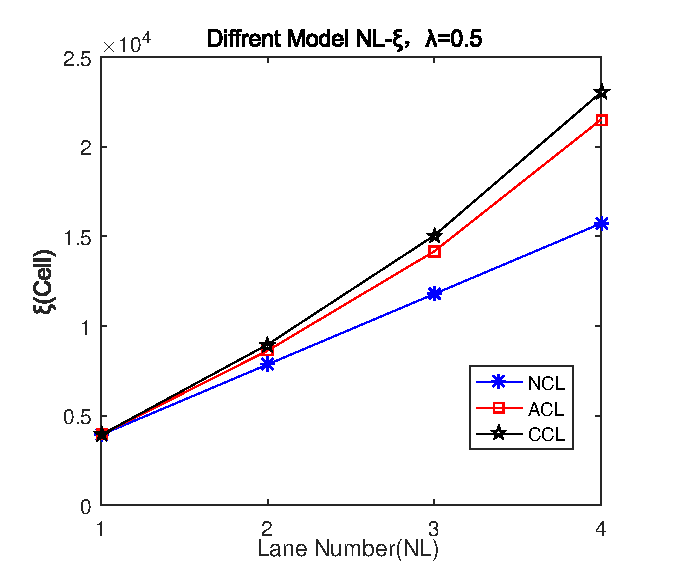
\includegraphics[width=8cm]{figure/421.eps}
\caption{a picture} \label{fig:a picture}
\end{figure}

%%插入两个并列图片4221和4222
\begin{figure}[H]
\centering
\subfigure[None dedicated lane]{
\label{figa} %% label for first subfigure
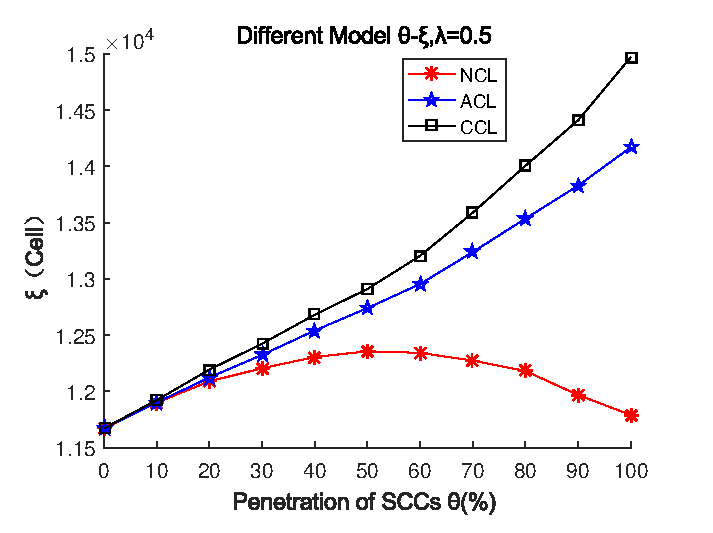
\includegraphics[width=5.3cm]{figure/4221.eps}}
\hspace{0cm}
\subfigure[Dedicated lane]{
\label{fig:subfig:b} %% label for second subfigure
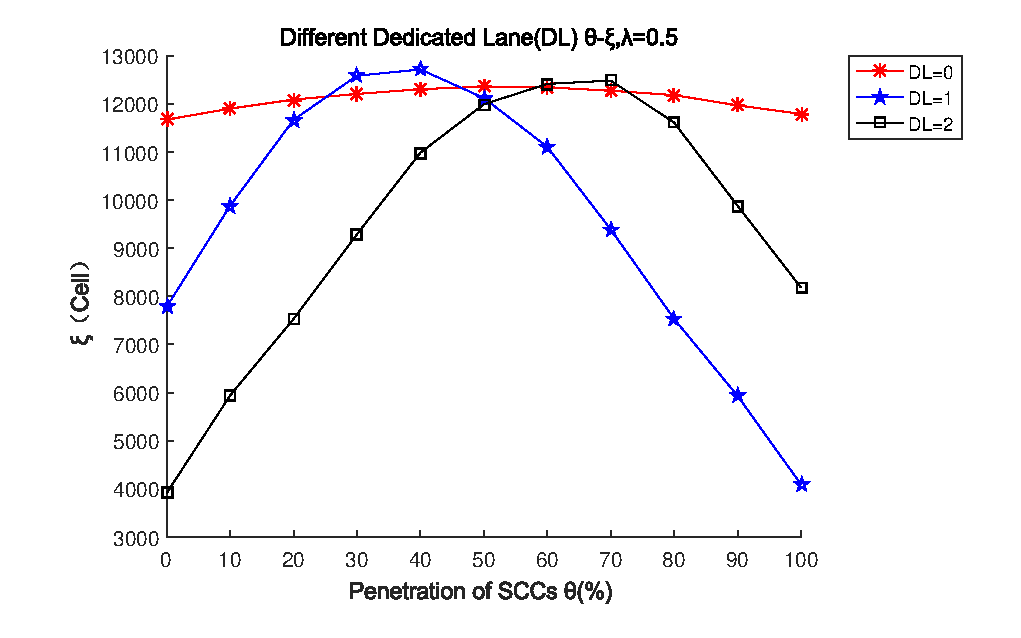
\includegraphics[width=6.6cm]{figure/4222.eps}}
\caption{Simulation Results for NCL,ACL,and CCL}
\label{figb} %% label for entire figure
\end{figure}


%%以下为定理代码
\begin{Theorem} 
for i>0, i++.
\end{Theorem}

%%以下为引理代码
\begin{Lemma} 
\TeX .
\end{Lemma}

\begin{Lemma} 
\TeX .
\end{Lemma}

\begin{Lemma} 
\TeX .
\end{Lemma}

\begin{Theorem} 
for i>0, i++.
\end{Theorem}

%%以下为证明
\begin{proof}
The proof of theorem.
\end{proof}

%%不一定要会,因为可以用mathtype写出公式之后导出latex代码
%%但是有时mathtype的公式导出时会出bug
%%所以建议还是看一看


%%公式输入,熟悉角标即可(常用)
%%    \]   和  $$  都是无编号的公式输入
%%      \begin{equation}  是有编号的输入
\begin{equation}
\sum\limits_{i = 1}^n {X_i^2} \sum\limits_{i = 1}^n {{X_i}{Y_i}} \frac{1}{n}\sum\limits_{i = 1}^n {{{({X_i} - \bar X)}^2}}       
\end{equation}

%%左对齐连续等号
\begin{equation}
\begin{array}{lllll}
 & \frac{{\delta y}}{{\delta x}}\\
{\rm{ = }} & \mathop {\lim }\limits_{\delta x \to 0} \\
{\rm{ = }} & \sum\limits_{i = 1}^n {{X_i}{Y_i}} \oint_S x dx\\
{\rm{ = }} & \sum\limits_{i = 1}^n {{{({X_i} - \bar X)}^2}} 
\end{array}
\end{equation}           %% 带上标号

%%矩阵
\[\left( {\begin{array}{*{20}{c}}
{{a_1}}&{}&0\\
{}& \ddots &{}\\
0&{}&{{a_n}}
\end{array}} \right)\left( {\begin{array}{*{20}{c}}
1&0\\
0&1
\end{array}} \right)\left( {\begin{array}{*{20}{c}}
{{a_{11}}}& \ldots &{{a_{1n}}}\\
 \vdots & \ddots & \vdots \\
{{a_{m1}}}& \cdots &{{a_{mn}}}
\end{array}} \right)\]


%%大括号分类
\[\left\{ \begin{array}{l}
ad\\
adf\\
adfa
\end{array} \right.\]

\begin{equation}
{p_{Lc,i}} = f({\delta _j},\tau ) = \left\{ \begin{array}{l}
1    ,{\delta _j} = 0\\
0   , {\delta _j} = 1\\
\max ( - \frac{\tau }{{1 - \tau }} \cdot {\delta _j} + 1,0){\rm{     }},otherwise{\rm{ }}
\end{array} \right.
\end{equation} 


\begin{equation}
{P_t}(n) = \frac{{{\lambda ^n}}}{{n!}}{e^{ - \lambda }}(n > 0)
\end{equation}
The $\lambda$ indicates the number of vehicles per unit time t. Let $ \lambda = \alpha t $, and $\alpha$ represents the average arrival rate of the vehicle. The Poisson distribution formula $(4.1)$ can be transformed into:
 \begin{equation}
{p_n}(t) = \frac{{{{(\alpha t)}^n}}}{{n!}}{e^{ - \alpha t}}(t > 0)
\end{equation}

%%无序列举
\begin{itemize}
\item  我的号哈佛的
\item  马上量很大
\item  撒考核法开始的恢复
\end{itemize}


%%加粗列举(看起来会很赞)
\begin{itemize}
\item \textbf{好的卡焦点科技几点开始}
\item \textbf{阿发达}
\item \textbf{看了就烦对哦}
\end{itemize}
%============= 参考文献 =====================
\addcontentsline{toc}{section}{参考文献}
\bibliography{bibfile}
\clearpage
%=============  致谢  ======================
\section*{致谢}
\addcontentsline{toc}{section}{致谢}
感谢父母为我提供的良好的衣食条件,让我有精力投入到这项没有经济回报的项目中去。
感谢徐海祥老师为我定制的论文题目,这个题目让我有兴趣制作这个模板。感谢武汉理工大学博士与硕士论文作者Hu,Weiyi,我在本模板制作的过程中参考了前辈的思路的方法。我研究过的模板还包括:上海交通大学,清华大学,哈尔滨工业大学,以及中国科技大学。其中论文引用格式GBT7714-2005-BibTeX-Style是上海财经大学的Haixing Hu作品,本模板离不开这些有益的资源的支持。同样感谢正在使用这个模板的你,相信通过你们的使用和传播,这个模板会变得越来越完善。
\newpage
\appendix

%%附录第一个章节
\section{第一附录}


%%变量列举

\begin{table}[H]
\caption{Symbol Table-Constants}
\centering
\begin{tabular}{lll}
\toprule
Symbol & Definition  & Units\\
\midrule[2pt]
\multicolumn{3}{c}{\textbf{Constants} }\\
$DL$&Expectancy of poisson-distribution &  unitless \\
$NCL$ &Never- Change-Lane& unitless\\
$CCL$&Cooperative-Change-Lane& unitless\\
$ACL$&Aggressive-Change-Lane& unitless\\
$FCL$&Friendly-Change-Lane& unitless\\
$SCC$&Self-driving-Cooperative-Car& unitless\\
$NSC$&None-Self-drive-Car& unitless\\
\bottomrule
\end{tabular}
\end{table}


\section{第二附录}
\textcolor[rgb]{0.98,0.00,0.00}{\textbf{Simulation Code}}
\begin{python}
import java.util.*;  
public class test {  
    public static void main (String[]args){   
        int day=0;  
        int month=0;  
        int year=0;  
        int sum=0;  
        int leap;     
        System.out.print("请输入年,月,日\n");     
        Scanner input = new Scanner(System.in);  
        year=input.nextInt();  
        month=input.nextInt();  
        day=input.nextInt();  
        switch(month) /*先计算某月以前月份的总天数*/    
        {     
        case 1:  
            sum=0;break;     
        case 2:  
            sum=31;break;     
        case 3:  
            sum=59;break;     
        case 4:  
            sum=90;break;     
        case 5:  
            sum=120;break;     
        case 6:  
            sum=151;break;     
        case 7:  
            sum=181;break;     
        case 8:  
            sum=212;break;     
        case 9:  
            sum=243;break;     
        case 10:  
            sum=273;break;     
        case 11:  
            sum=304;break;     
        case 12:  
            sum=334;break;     
        default:  
            System.out.println("data error");break;  
        }     
        sum=sum+day; /*再加上某天的天数*/    
        if(year%400==0||(year%4==0&&year%100!=0))/*判断是不是闰年*/    
            leap=1;     
        else    
            leap=0;     
        if(leap==1 && month>2)/*如果是闰年且月份大于2,总天数应该加一天*/    
            sum++;     
        System.out.println("It is the the day:"+sum);  
        }  
} 
\end{python}




\end{document}
%%%%%%%%%% 结束 %%%%%%%%%%